\documentclass[12pt]{article}
\usepackage{tabularx} % extra features for tabular environment
\usepackage{amsmath}  % improve math presentation
\usepackage{graphicx} % takes care of graphic including machinery
\usepackage[margin=1in,letterpaper]{geometry} % decreases margins
\usepackage{cite} % takes care of citations
\usepackage[final]{hyperref} % adds hyper links inside the generated pdf file
\usepackage{mathtools}
\usepackage[utf8]{inputenc}

\usepackage{listings}
\usepackage{xcolor}

%New colors defined below
\definecolor{codegreen}{rgb}{0,0.6,0}
\definecolor{codegray}{rgb}{0.5,0.5,0.5}
\definecolor{codepurple}{rgb}{0.58,0,0.82}
\definecolor{backcolour}{rgb}{0.95,0.95,0.92}

%Code listing style named "mystyle"
\lstdefinestyle{mystyle}{
  backgroundcolor=\color{backcolour},   commentstyle=\color{codegreen},
  keywordstyle=\color{magenta},
  numberstyle=\tiny\color{codegray},
  stringstyle=\color{codepurple},
  basicstyle=\ttfamily\footnotesize,
  breakatwhitespace=false,         
  breaklines=true,                 
  captionpos=b,                    
  keepspaces=true,                 
  numbers=left,                    
  numbersep=5pt,                  
  showspaces=false,                
  showstringspaces=false,
  showtabs=false,                  
  tabsize=2
}

%"mystyle" code listing set
\lstset{style=mystyle}


\DeclarePairedDelimiter\floor{\lfloor}{\rfloor}

\hypersetup{
	colorlinks=true,       % false: boxed links; true: colored links
	linkcolor=blue,        % color of internal links
	citecolor=blue,        % color of links to bibliography
	filecolor=magenta,     % color of file links
	urlcolor=blue         
}
\usepackage{blindtext}
%++++++++++++++++++++++++++++++++++++++++


\begin{document}
\title{Generating Discrete Random Numbers Using Poisson Distribution}
\author{Shamiul Hasan\\1505038}
\date{\today}
\maketitle


\section{Problem Description}
In probability theory and statistics, the Poisson distribution is a discrete probability distribution that expresses the probability of a given number of events occurring in a fixed interval of time or space if these events occur with a known constant mean rate and independently of the time since the last event. The Poisson distribution can also be used for the number of events in other specified intervals such as distance, area or volume.
In this assignment, we have to generate N number of random variables using the Poisson Distribution. We also have to show the curve plotting the probability distribution and observed frequencies in fraction (frequency/N) i.e. observed probability. For this problem, the parameter $\lambda = 1$.


\section{Definitions}

A discrete random variable $X$ is said to have a Poisson distribution with parameter $\lambda > 0$, if, for $k = 0, 1, 2, \cdots$ the probability mass function of $X$ is given by, \\

\begin{equation}
	Mass, p(x)=
	\begin{cases}
		{\frac {e^{-\lambda}\lambda ^{x}}{x!}}, & \text{if}\ x \epsilon \{0,1,2,\cdots\} \\ \\
		0,                                      & \text{otherwise}
	\end{cases}
\end{equation}


\begin{equation}
	Distribution,F(x)=
	\begin{cases}
		{\frac {e^{-\lambda}\lambda ^{x}}{x!}}, & \text{if}\ x < 0 \\ \\
		e^{-\lambda}\sum_{i=0}^{\floor*{x}}2,   & \text{otherwise}
	\end{cases}
\end{equation}

\clearpage

\section{Code}
Below is the Python code to simulate this problem. 
\lstinputlisting[language=Python, 
caption=Python Code
]{../Poisson.py}
\begin{figure}[!h]
	\centering
	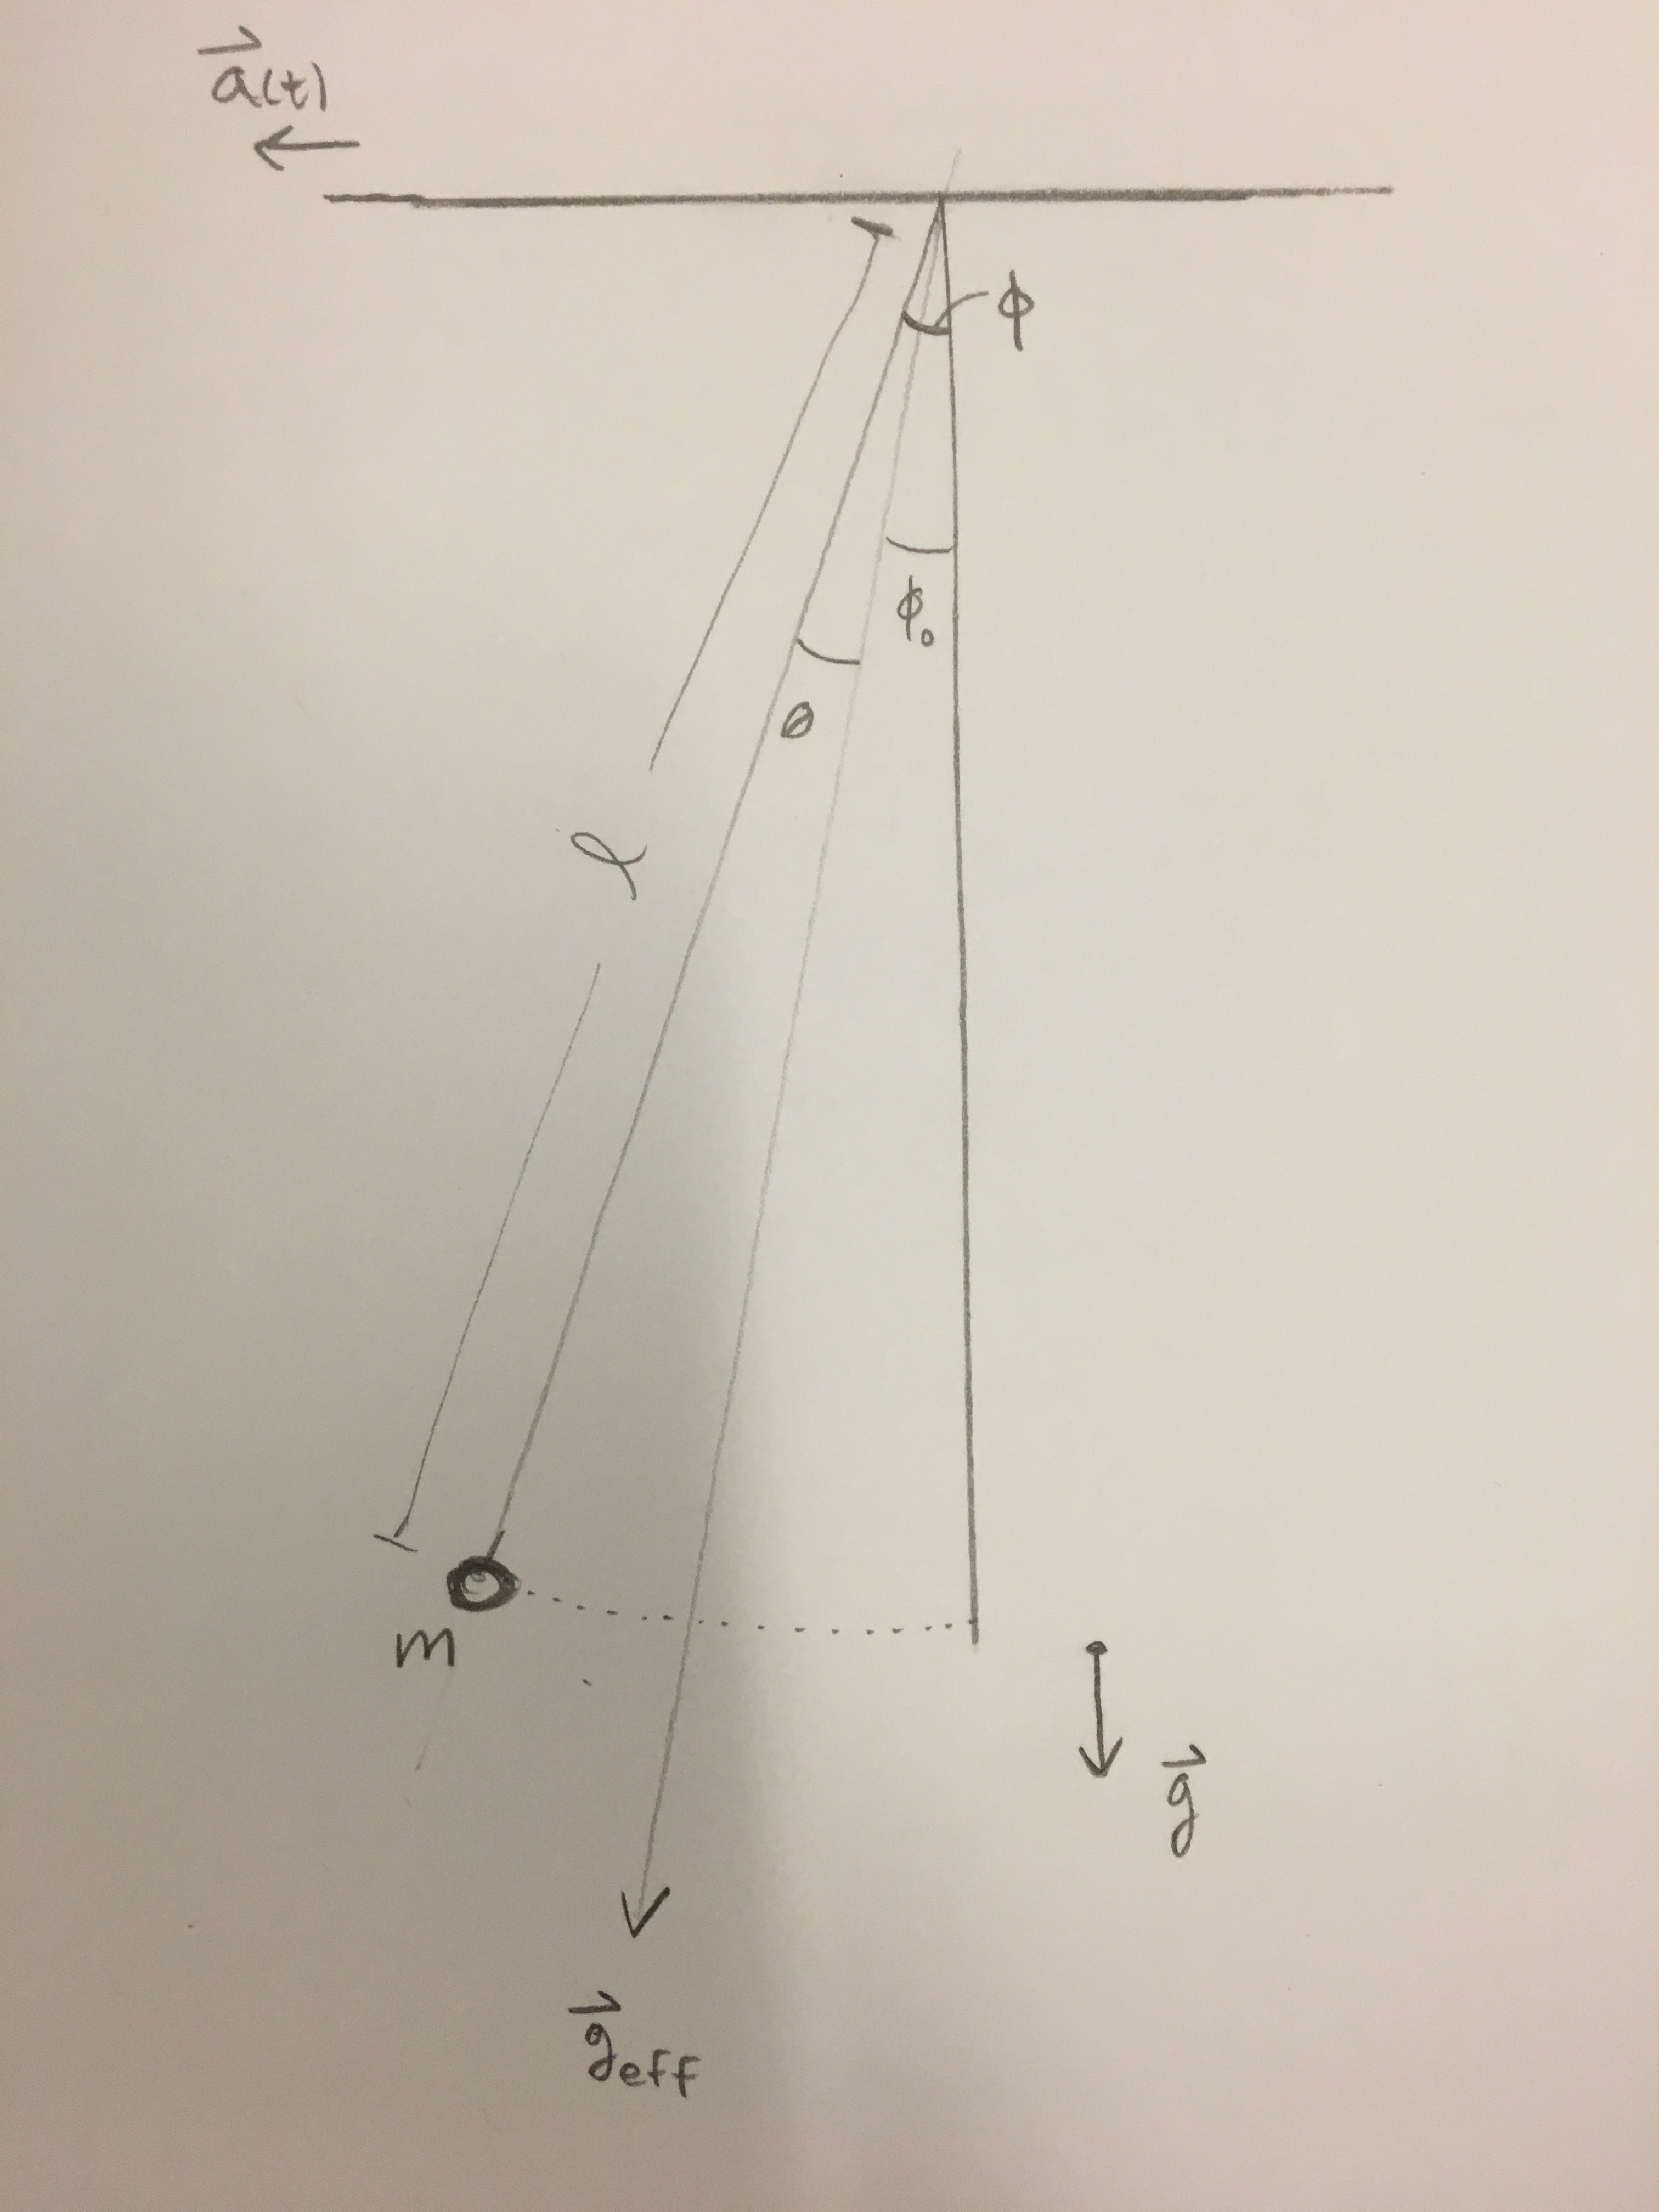
\includegraphics[width=.8\textwidth]{pendulum.jpg}
	\caption{Pendulum that starts at rest in an accelerating frame. If the acceleration is not constant then the apparent vertical, and thus $\phi_0$ will change with time}
\end{figure}

\section{Results}


Give a schematic of the experimental setup(s) used in the experiment (see
figure~\ref{fig:samplesetup}). Give the description of  abbreviations
either in the figure caption or in the text. Write a description of what is
going on.


and eventually arrived to the
balanced photodiode as seen in the figure~\ref{fig:samplesetup}.


\section{Results}

In this section you will need to show your experimental results. Use tables and
graphs when it is possible. Table~\ref{tbl:bins} is an example.

\begin{table}[ht]
	\begin{center}
		\caption{Every table needs a caption.}
		\label{tbl:bins} % spaces are big no-no withing labels
		\begin{tabular}{|cc|}
			\hline
			\multicolumn{1}{|c}{$x$ (m)} & \multicolumn{1}{c|}{$V$ (V)} \\
			\hline
			0.0044151                    & 0.0030871                    \\
			0.0021633                    & 0.0021343                    \\
			0.0003600                    & 0.0018642                    \\
			0.0023831                    & 0.0013287                    \\
			\hline
		\end{tabular}
	\end{center}
\end{table}

Analysis of equation~\ref{eq:equation1} shows ...

\blindtext

\begin{figure}
	\centering
	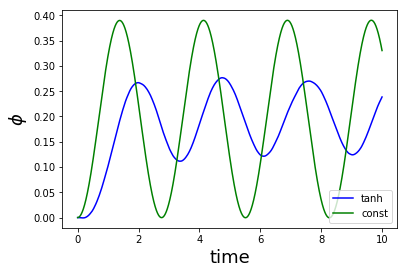
\includegraphics[width=.7\textwidth]{tanh_vs_const_1.png}
	\caption{Hyperbolic tangent acceleration vs immediate constant acceleration. The slow approach to the same asymptotic value of 2 meters per second per second induces a lag in the oscillation and also diminishes the amplitude of oscillation.}
\end{figure}

For example, it is easy to conclude that the
experiment and theory match each other rather well if you look at
Fig.~\ref{fig:samplesetup} and Fig.~\ref{fig:exp_plots}.


\section{Conclusions}
Here you briefly summarize your findings. Did you learn any new physics? Was everything as expected?

\blindtext

\section{Future Work}
Since you had limited time to work on this project, what questions are left outstanding? What would be your next steps?

\blindtext

%++++++++++++++++++++++++++++++++++++++++
% References section will be created automatically 
% with inclusion of "thebibliography" environment
% as it shown below. See text starting with line
% \begin{thebibliography}{99}
% Note: with this approach it is YOUR responsibility to put them in order
% of appearance.

\begin{thebibliography}{99}

	\bibitem{melissinos}
	A.~C. Melissinos and J. Napolitano, \textit{Experiments in Modern Physics},
	(Academic Press, New York, 2003).

	\bibitem{Cyr}
	N.\ Cyr, M.\ T$\hat{e}$tu, and M.\ Breton,
	% "All-optical microwave frequency standard: a proposal,"
	IEEE Trans.\ Instrum.\ Meas.\ \textbf{42}, 640 (1993).

	\bibitem{Wiki} \emph{Expected value},  available at
	\texttt{http://en.wikipedia.org/wiki/Expected\_value}.

\end{thebibliography}


\end{document}
